\documentclass[dvipdfmx]{jsarticle}
\usepackage{geometry}
\geometry{a4paper, top=1.0cm, left=2.5cm, right=2.5cm, bottom=1cm, includefoot}

\usepackage[dvipdfmx]{graphicx, xcolor}
\usepackage{here}
\usepackage{color}
\usepackage{xcolor}
\usepackage{amsmath, amssymb, bm}
\usepackage{amsthm}
\usepackage{cases}
\usepackage{cite}
\usepackage{enumitem}
\usepackage{mathtools}
\usepackage{multirow}
\usepackage{bbm}
\usepackage{ascmac}
\usepackage{arydshln}
\usepackage[table]{xcolor}
\usepackage{float}
\usepackage{fancybox}
\usepackage{caption}
\usepackage{mdframed}
\usepackage{hyperref}
\usepackage{algorithm,algorithmic}
\usepackage{wrapfig}
\usepackage{url}
\usepackage{indentfirst}
\usepackage{stmaryrd}
\usepackage{braket}
\usepackage{booktabs}
\usepackage{siunitx} % 数値列の整列に便利
\usepackage{mathcomp}
\usepackage{subfig}


\graphicspath{{fig/}}
%\usepackage{color}
\captionsetup{justification=centering}

\newtheorem{theorem}{定理}
\newtheorem{lemma}[theorem]{補題}
\renewcommand{\figurename}{図}
\renewcommand{\abstractname}{Abstract}
\newcommand{\la}{\lambda}
\newcommand{\li}{\lambda_i}
\newcommand{\argmax}{\mathop{\rm arg~max}\limits}
\newcommand{\argmin}{\mathop{\rm arg~min}\limits}

\newcommand{\ds}{\displaystyle}
\newcommand{\dd}{\mathrm{d}}
\newcommand{\E}{\mathrm{E}}
\newcommand{\one}{\mathbbm{1}}
\newcommand{\bb}{\mathbb{R}}

\DeclareGraphicsRule{.tif}{png}{.png}{`convert #1 `dirname #1`/`basename #1 .tif`.png}
% Vectors

\newcommand{\av}{\mathbf{a}}
\newcommand{\bv}{\mathbf{b}}
\newcommand{\cv}{\mathbf{c}}
\newcommand{\dv}{\mathbf{d}}
\newcommand{\ev}{\mathbf{e}}
\newcommand{\fv}{\mathbf{f}}
\newcommand{\gv}{\mathbf{g}}
\newcommand{\hv}{\mathbf{h}}
\newcommand{\iv}{\mathbf{i}}
\newcommand{\jv}{\mathbf{j}}
\newcommand{\kv}{\mathbf{k}}
\newcommand{\lv}{\mathbf{l}}
\newcommand{\mv}{\mathbf{m}}
\newcommand{\nv}{\mathbf{n}}
\newcommand{\ov}{\mathbf{o}}
\newcommand{\pv}{\mathbf{p}}
\newcommand{\qv}{\mathbf{q}}
\newcommand{\rv}{\mathbf{r}}
\newcommand{\sv}{\mathbf{s}}
\newcommand{\tv}{\mathbf{t}}
\newcommand{\uv}{\mathbf{u}}
\newcommand{\wv}{\mathbf{w}}
\newcommand{\vv}{\mathbf{v}}
\newcommand{\xv}{\mathbf{x}}
\newcommand{\yv}{\mathbf{y}}
\newcommand{\zv}{\mathbf{z}}
\newcommand{\zerov}{\mathbf{0}}
\newcommand{\onev}{\mathbf{1}}

% Matrices

\newcommand{\Am}{\mathbf{A}}
\newcommand{\Bm}{\mathbf{B}}
\newcommand{\Cm}{\mathbf{C}}
\newcommand{\Dm}{\mathbf{D}}
\newcommand{\Em}{\mathbf{E}}
\newcommand{\Fm}{\mathbf{F}}
\newcommand{\Gm}{\mathbf{G}}
\newcommand{\Hm}{\mathbf{H}}
\newcommand{\Id}{\mathbf{I}}
\newcommand{\Jm}{\mathbf{J}}
\newcommand{\Km}{\mathbf{K}}
\newcommand{\Lm}{\mathbf{L}}
\newcommand{\Mm}{\mathbf{M}}
\newcommand{\Nm}{\mathbf{N}}
\newcommand{\Om}{\mathbf{O}}
\newcommand{\Pm}{\mathbf{P}}
\newcommand{\Qm}{\mathbf{Q}}
\newcommand{\Rm}{\mathbf{R}}
\newcommand{\Sm}{\mathbf{S}}
\newcommand{\Tm}{\mathbf{T}}
\newcommand{\Um}{\mathbf{U}}
\newcommand{\Wm}{\mathbf{W}}
\newcommand{\Vm}{\mathbf{V}}
\newcommand{\Xm}{\mathbf{X}}
\newcommand{\Ym}{\mathbf{Y}}
\newcommand{\Zm}{\mathbf{Z}}
\newcommand{\Lam}{\mathbf{\Lambda}}

% Calligraphic
\newcommand{\Ac}{\mathcal{A}}
\newcommand{\Bc}{\mathcal{B}}
\newcommand{\Cc}{\mathcal{C}}
\newcommand{\Dc}{\mathcal{D}}
\newcommand{\Ec}{\mathcal{E}}
\newcommand{\Fc}{\mathcal{F}}
\newcommand{\Gc}{\mathcal{G}}
\newcommand{\Hc}{\mathcal{H}}
\newcommand{\Ic}{\mathcal{I}}
\newcommand{\Jc}{\mathcal{J}}
\newcommand{\Kc}{\mathcal{K}}
\newcommand{\Lc}{\mathcal{L}}
\newcommand{\Mc}{\mathcal{M}}
\newcommand{\Nc}{\mathcal{N}}
\newcommand{\Oc}{\mathcal{O}}
\newcommand{\Pc}{\mathcal{P}}
\newcommand{\Qc}{\mathcal{Q}}
\newcommand{\Rc}{\mathcal{R}}
\newcommand{\Sc}{\mathcal{S}}
\newcommand{\Tc}{\mathcal{T}}
\newcommand{\Uc}{\mathcal{U}}
\newcommand{\Wc}{\mathcal{W}}
\newcommand{\Vc}{\mathcal{V}}
\newcommand{\Xc}{\mathcal{X}}
\newcommand{\Yc}{\mathcal{Y}}
\newcommand{\Zc}{\mathcal{Z}}
\newcommand{\Ecb}{\mathbf{\mathcal{E}}}
\newcommand{\Ocb}{\mathbf{\mathcal{O}}}
\newcommand{\Lcb}{{\bm \mathcal{L}}}

% Bold greek letters

\newcommand{\alphav}{\hbox{\boldmath$\alpha$}}
\newcommand{\betav}{\hbox{\boldmath$\beta$}}
\newcommand{\gammav}{\hbox{\boldmath$\gamma$}}
\newcommand{\deltav}{\hbox{\boldmath$\delta$}}
\newcommand{\etav}{\hbox{\boldmath$\eta$}}
\newcommand{\lambdav}{\hbox{\boldmath$\lambda$}}
\newcommand{\epsilonv}{\hbox{\boldmath$\epsilon$}}
\newcommand{\nuv}{\hbox{\boldmath$\nu$}}
\newcommand{\muv}{\hbox{\boldmath$\mu$}}
\newcommand{\zetav}{\hbox{\boldmath$\zeta$}}
\newcommand{\phiv}{\hbox{\boldmath$\phi$}}
\newcommand{\psiv}{\hbox{\boldmath$\psi$}}
\newcommand{\thetav}{\hbox{\boldmath$\theta$}}
\newcommand{\tauv}{\hbox{\boldmath$\tau$}}
\newcommand{\omegav}{\hbox{\boldmath$\omega$}}
\newcommand{\xiv}{\hbox{\boldmath$\xi$}}
\newcommand{\sigmav}{\hbox{\boldmath$\sigma$}}
\newcommand{\piv}{\hbox{\boldmath$\pi$}}
\newcommand{\rhov}{\hbox{\boldmath$\rho$}}

\newcommand{\Gammam}{\hbox{\boldmath$\Gamma$}}
\newcommand{\Lambdam}{\hbox{\boldmath$\Lambda$}}
\newcommand{\Deltam}{\hbox{\boldmath$\Delta$}}
\newcommand{\Sigmam}{\hbox{\boldmath$\Sigma$}}
\newcommand{\Phim}{\hbox{\boldmath$\Phi$}}
\newcommand{\Pim}{\hbox{\boldmath$\Pi$}}
\newcommand{\Psim}{\hbox{\boldmath$\Psi$}}
\newcommand{\Thetam}{\hbox{\boldmath$\Theta$}}
\newcommand{\Omegam}{\hbox{\boldmath$\Omega$}}
\newcommand{\Xim}{\hbox{\boldmath$\Xi$}}

% mixed symbols

% \newcommand{\sinc}{{\hbox{sinc}}}
% \newcommand{\diag}{{\hbox{diag}}}
% \renewcommand{\det}{{\hbox{det}}}
% \newcommand{\trace}{{\hbox{tr}}}
% \newcommand{\sign}{{\hbox{sign}}}
% \renewcommand{\arg}{{\hbox{arg}}}
% \newcommand{\var}{{\hbox{var}}}
% \newcommand{\cov}{{\hbox{cov}}}
% \newcommand{\SINR}{{\sf SINR}}
% \newcommand{\SNR}{{\sf SNR}}
% \newcommand{\Ei}{{\rm E}_{\rm i}}
% \renewcommand{\Re}{{\rm Re}}
% \renewcommand{\Im}{{\rm Im}}
% \newcommand{\eqdef}{\stackrel{\Delta}{=}}
% \newcommand{\defines}{{\,\,\stackrel{\scriptscriptstyle \bigtriangleup}{=}\,\,}}
% \newcommand{\<}{\left\langle}
% \renewcommand{\>}{\right\rangle}
% \newcommand{\herm}{{\sf H}}
% \newcommand{\transp}{{\sf T}}
% \renewcommand{\vec}{{\rm vec}}


% New theorem environments
% \newtheorem{theorem}{Theorem}
% \newtheorem{conjecture}{Conjecture}
% \newtheorem{proposition}{Proposition}
% \newtheorem{lemma}{Lemma}
% \newtheorem{definition}{Definition}
% \newtheorem{corollary}{Corollary}
% \newtheorem{objective}{Objective}
% \newtheorem{observation}{Observation}

% \newcommand{\E}[1]{\mathbb{E}\left\{{#1}\right\}}
% \newcommand{\Var}[1]{\text{Var}\left\{{#1}\right\}}
% \newcommand{\Tr}[1]{\text{Tr}\left({#1}\right)}
% \newcommand{\defeq}{\stackrel{\triangle}{=}}


% \DeclareMathOperator*{\argmin}{arg\,min}
% \DeclareMathOperator*{\argmax}{arg\,max}




\title{進捗報告}
\author{林 奏汰}
\date{2026/4/10}

\begin{document}

\maketitle


% \begin{abstract}
% 人は，環境に潜む規則性を意識せずとも自然に習得する能力を有しており，これは暗黙的学習と呼ばれる．
% 前回の進捗報告では，反応時間の変動係数を注意状態の個人差指標として用い，学習指標との関係を検討した．
% その結果，注意状態が不安定な参加者ほど暗黙的学習の進行が促進されることが示唆された．
% 本報告では，そのメカニズムとして試行レベルの注意変動が媒介している可能性について検討する．
% 具体的には，反応時間の時系列から試行ごとの注意状態をラベル付けし，Q学習モデルを用いて注意状態ごとに学習の進行度合いを定量化することを試みた．
% その結果，注意が散漫状態における学習率は集中状態よりも高い傾向が認められたが，その差分と反応時間の変動係数との間に有意な関係は確認されなかった．
% \end{abstract}

\section{\textcolor{red}{イントロダクション}}
人は，環境に潜む規則性を意識せずとも自然に習得する能力を有している．
これは暗黙的学習と呼ばれ，言語習得や運動技能の獲得など，様々な場面で重要な役割を果たしている~\cite{cleeremans1998implicit,frensch2003implicit,maresch2021measures,costea2023implicit}．

暗黙的な規則性の習得過程には顕著な個人差が認められる~\cite{kalra2019evidence}．
前回の進捗報告では，反応時間の変動係数を注意状態の個人差指標として用い，学習指標との関係を検討した．
その結果，反応時間の変動係数が大きい参加者ほど，課題の進行にともない高報酬なドット群を選択する割合が有意に増加することが確認された．
この結果は，注意状態の変動が暗黙的学習の進行に影響していることを示唆している．
本報告では，そのメカニズムとして試行レベルの注意変動が媒介している可能性について検討する．

あるマインドワンダリング研究では，反応時間の時系列から試行ごとの注意状態をラベル付けする手法が提案されている~\cite{decker2023pay}．
この手法では，直前数試行の反応時間の移動平均が個人平均より短く，かつ局所的な変動が大きい試行を散漫状態（Out Of the Zone: OOZ）と定義し，試行ごとに注意状態を決定する．
試行レベルの注意変動が学習を媒介しているかを検証するためには，注意状態ごとの学習の進行度合いを比較する必要がある．
そこで本報告では，Q学習モデルを用いて注意状態ごとの学習率を推定し，OOZ状態とNon-OOZ状態で学習の進行度合いが異なるかを検討した．
さらに，その学習率の差分が反応時間の変動係数と関連するかについても検討した．

その結果，OOZ状態における学習率はNon-OOZ状態よりも高い傾向が認められたが，
その差分と反応時間の変動係数との間に有意な関係は確認されなかった．
この結果は，試行レベルの注意変動と個人レベルの注意特性が暗黙的学習に対して独立に寄与している可能性を示唆している．


\section{実験}
\begin{figure}[t]
    \centering
    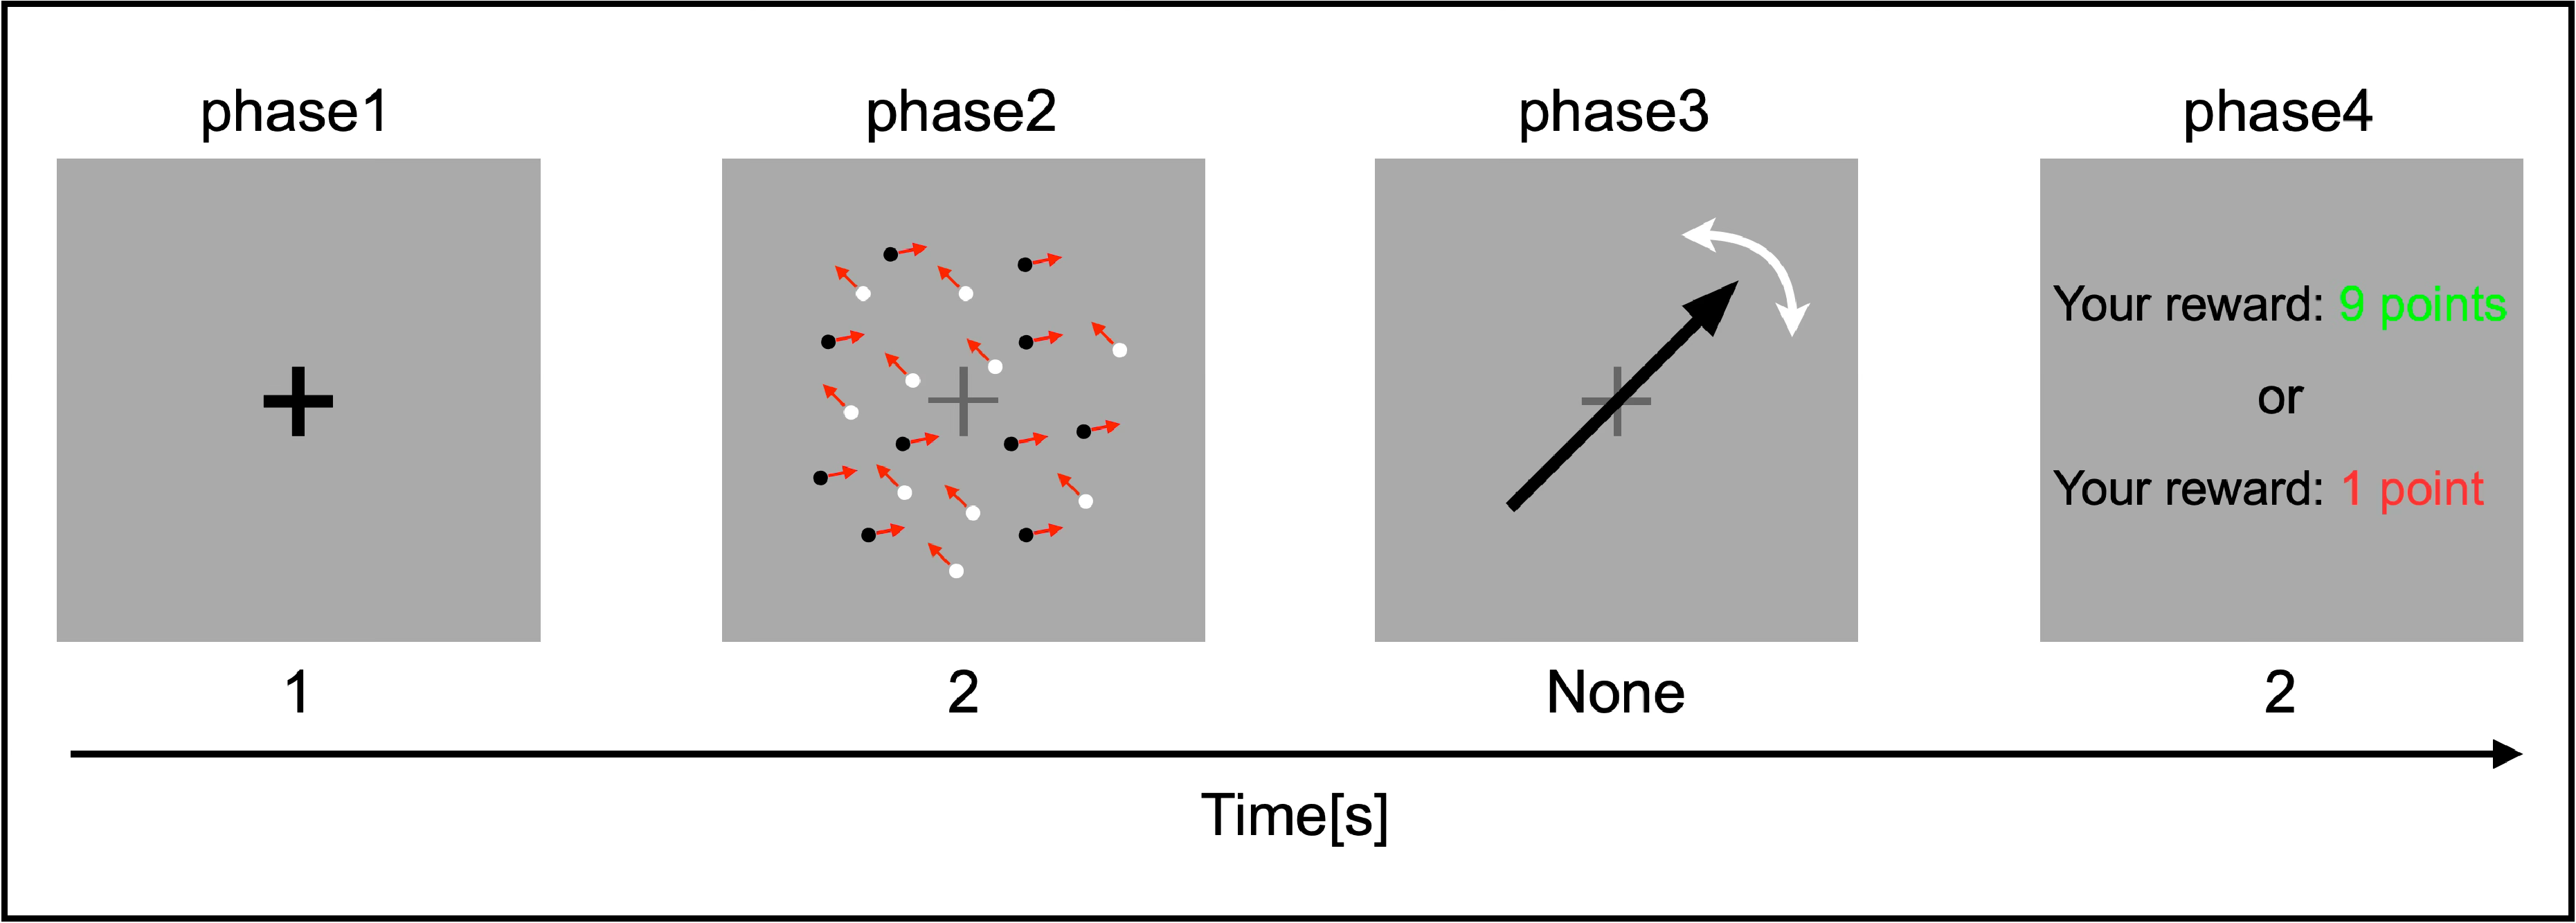
\includegraphics[width=1.0\textwidth]{../fig/dual-rdk-procedure-modified.pdf}
    \caption{実験の1回の試行の流れ．}
    \label{fig:experiment_procedure}
\end{figure}

\subsection{環境}
実験は，JsPsych v2.0.0を用いて作成した．

\subsection{実験参加者}
実験参加者は合計80名で，オンライン実験ツールであるProlific~\cite{palan2018prolific}を用いて募集した．

\subsection{実験手順}
実験は16試行の練習セッションと72試行の本番セッションで構成された．
実験の1回の試行を図~\ref{fig:experiment_procedure}に示す．
1試行は，固視点の提示，色（白・黒）の異なる2つのRDK刺激の同時提示，方向の回答フェーズ，そして報酬フェーズで構成された．

実験参加者には，白・黒のドット群がそれぞれ異なる方向に運動する2種類のRDK刺激を同時に提示し，
ドット数の多い方のドット群の運動方向を報告するように指示した．
つまり，この課題では，ドット数の多い刺激がターゲット刺激であり，ドット数の少ない刺激がディストラクタ刺激であった．
各試行は固視点提示（1秒），刺激提示（2秒），回答，報酬提示（2秒）の4つのフェーズで構成された．
固視点は参加者の視線を画面中央に誘導し，刺激提示前の視線のばらつきを抑制することを目的とした．
刺激提示フェーズでは白・黒のRDK刺激を同時に提示し，
回答フェーズでは，参加者には，キーボードの左右の矢印キーを用いてバーを回転させ，
その向きをドット群の運動方向に一致させるように指示した．
バーの初期位置はランダムに決定され，回答時間は無制限であった．
報酬フェーズではターゲット刺激に対する角度誤差に応じた報酬を提示した
（報酬の決定方法については\ref{sec:reward_structure}節で述べる）．
参加者には，最終的な獲得報酬に応じて実験終了後に謝金が支払われることを事前に伝えた．
実験が終了するまで約15分を要した．

\subsubsection{練習セッション}
練習セッションは16試行で構成され，バーの操作に慣れてもらうという目的のもと，
ドット数と方向はランダムに決定し，2つの輝度の異なるRDK刺激を同時表示した．
したがって，練習セッションでは，2つのドット群のドット数の差が顕著に現れる．

\subsubsection{本番セッション}
本番セッションは72試行で構成され，前半48試行はlearningステージ，後半24試行はawarenessステージとした．
本番セッションの各試行では，ドット数が同数である2つの色の異なるRDK刺激を同時表示した．
つまり，2つのRDK刺激のドット数は同数であるため，ターゲット刺激とディストラクタ刺激の区別はない．
ただし，ドット群が運動する方向は2色のドット群でそれぞれ異なり，その運動方向に応じて報酬が変化するように設定した．
したがって，本番セッションでは，参加者はドット数が多いと感じた方のドット群の運動方向を報告することを指示されたが，
実際にはドット数ではなく，運動方向によって得られる報酬が変化した．
次節では，本番セッションにおける報酬構造について述べる．


\subsection{報酬構造}\label{sec:reward_structure}
実験の本番セッションにおける報酬構造は，参加者には明示的に伝えられておらず，
報酬をより多く獲得するためには，暗黙的に設定された報酬構造を学習する必要がある．

\begin{figure}[t]
    \centering
    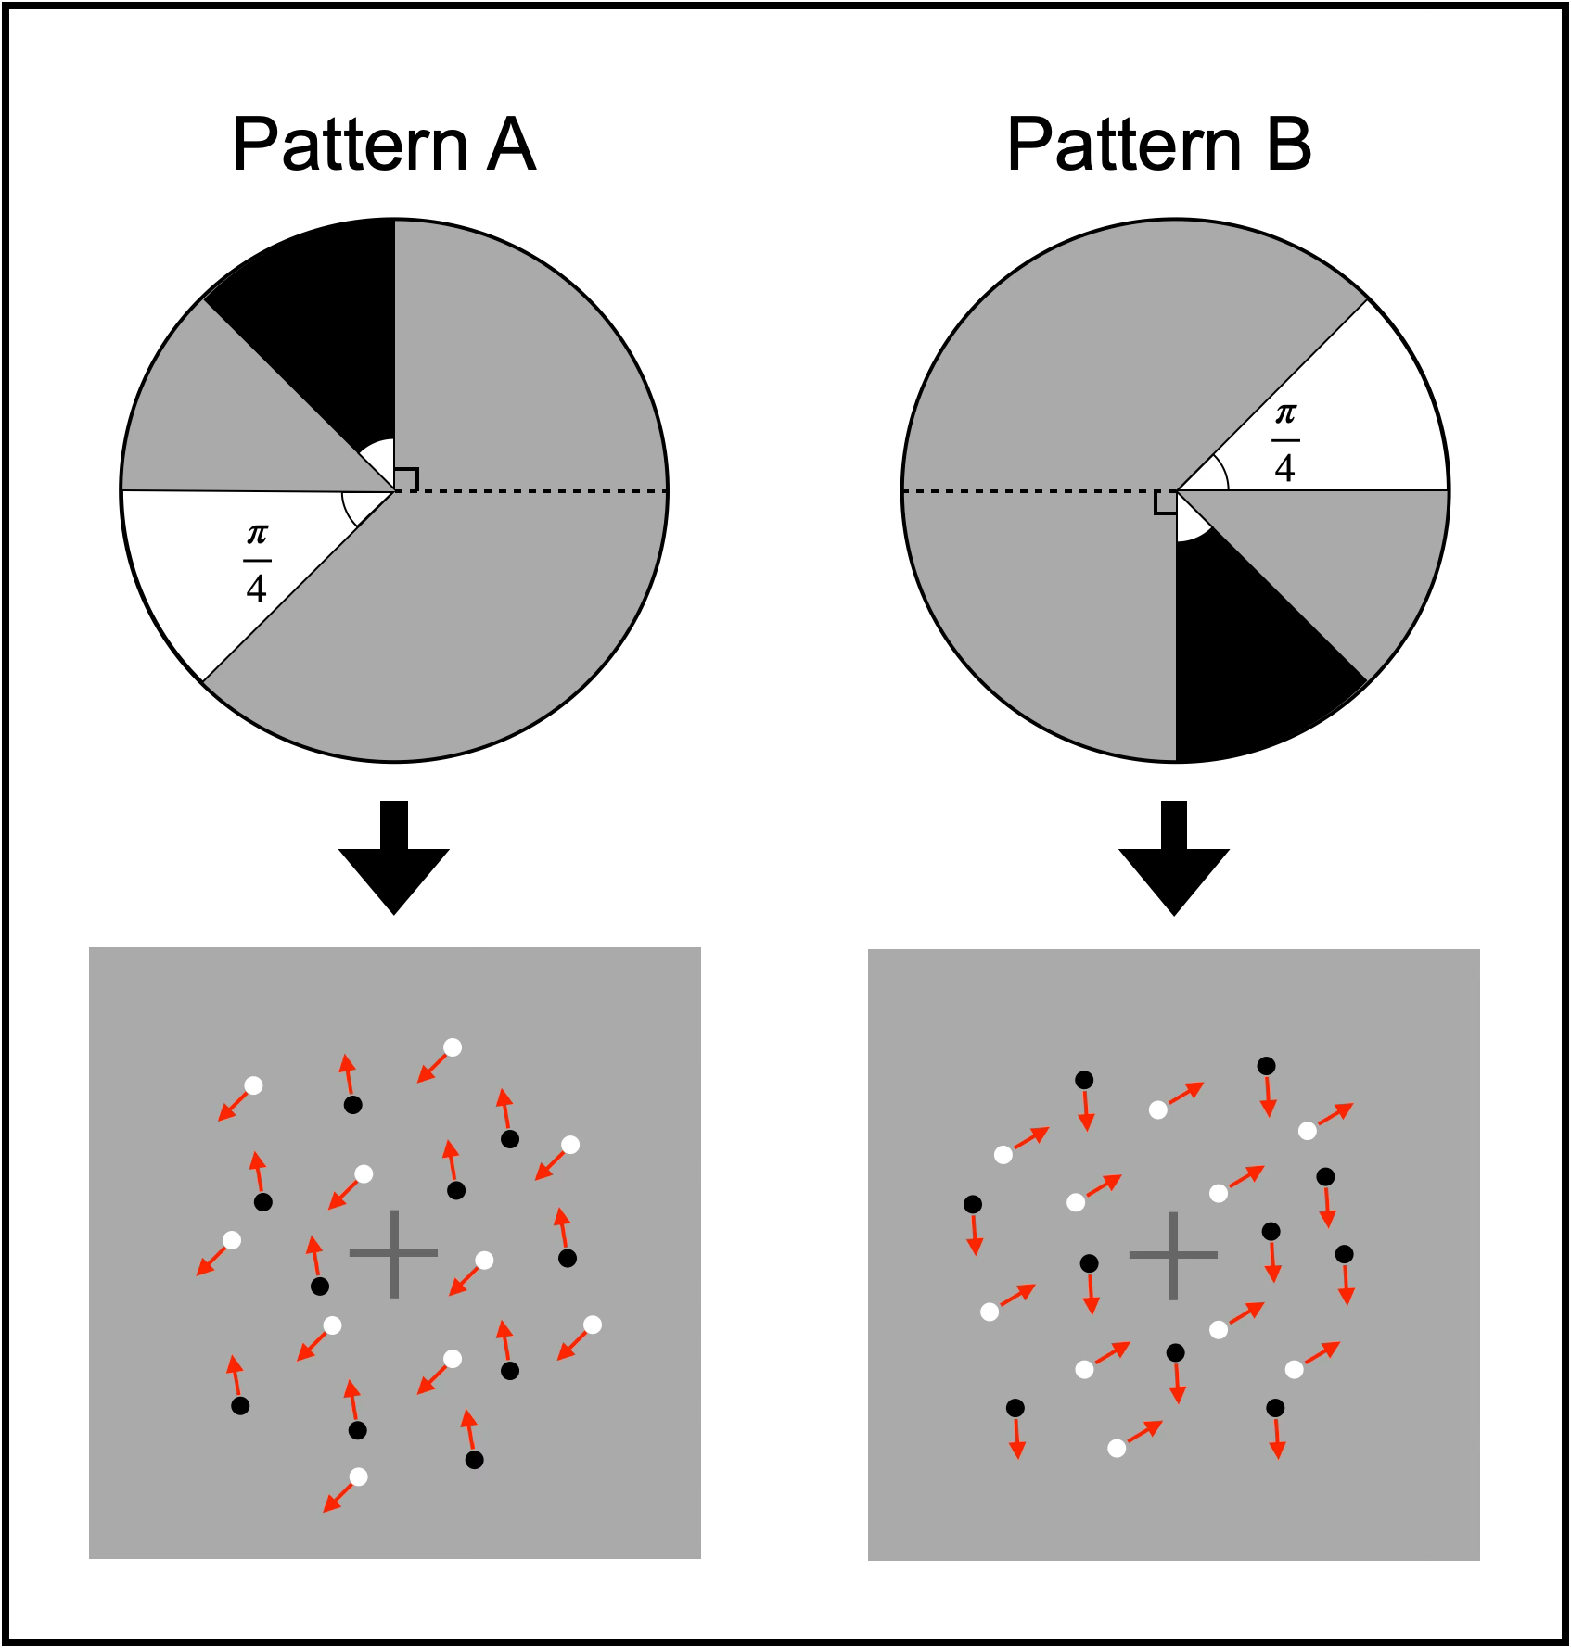
\includegraphics[width=0.5\linewidth]{../fig/learning-stimuli-modified.pdf}
    \caption{本番セッションにおける2種類の刺激パターン．
    （上段）白・黒のドット群の運動方向の発生範囲．
    （下段）刺激の具体例（赤矢印はドット群の運動方向を示す）．
    % 右側のペアの場合は白色ドット群がターゲット，黒色ドット群がディストラクタとなる\\
    % 左側は黒色ドット群がターゲット，白色ドット群がディストラクタとなる
    }
    \label{fig:stimuli}
\end{figure}
本番セッションの各試行における刺激は，高報酬刺激と低報酬刺激で構成された．
それぞれ高報酬刺激と低報酬刺激は運動方向に規則性があり，そのパターンが2種類存在した．
図~\ref{fig:stimuli}は，本番セッションにおける2種類の刺激のパターン，ドット群の運動方向の範囲，および刺激の具体例を示す．
パターンAでは，高報酬刺激は黒色ドット群であり，低報酬刺激は白色ドット群である．
逆にパターンBでは，高報酬刺激は白色ドット群であり，低報酬刺激は黒色ドット群である．
各試行では，これら2種類の刺激のパターンのうちどちらかがランダムに選択されて提示された．
それぞれの刺激の運動方向の発生範囲は$\pi/4$で，高報酬刺激と低報酬刺激の発生範囲間の角度距離は$\pi/4$である．

各試行の報酬は，回答角度がターゲットの方向角度に一致すると10点，$\pi/4$以上離れると0点になるように調整した．
これを実現するため，各試行において2つのドット群の運動方向のなす角度が常に$\pi/2$以上になるように制限を加えた．
これにより，参加者がターゲットを正確に報告した場合でも，
その回答がディストラクタの方向と混同されないことが保証される．

\subsection{ステージの設計}
本節では，本番セッションにおけるlearningステージとawarenessステージの設計について説明する．

learningステージでは，参加者が報酬構造を暗黙的に学習するかどうかを検証することを目的とした．
参加者には報酬構造の存在を明示せず，試行を重ねることで高報酬なドット群を選択する割合が増加するかどうかを学習指標として用いた．

awarenessステージでは，learningステージで生じた学習が意識的な知識に基づくものかどうかを検証することを目的とした．
そのため，awarenessステージにおける報酬構造は，
learningステージのものを極座標の角度方向に$\pi$回転させたもの，
すなわち高報酬と低報酬のドット群が入れ替わった構造とした．
learningステージで獲得した知識が意識的なものであれば，報酬構造の反転に気づき選択行動が変化すると予測される．
一方，学習が無意識的なものであれば，報酬構造の反転後も以前の選択傾向が持続すると予測される．

以降の分析では，本番セッションにおける高報酬刺激を
便宜上ターゲット刺激と呼び，
高報酬刺激を選択した割合をターゲット選択率と定義する．


\section{\textcolor{red}{計算論的枠組み}}
本研究では，先行研究~\cite{decker2023pay}の手法を参考に，反応時間の時系列から試行ごとの注意状態をラベル付けし，
さらにQ学習モデルを用いて注意状態ごとに学習の進行度合いを定量化することを試みた．

\subsection{注意状態のラベル付け}\label{sec:attention_labeling}
deckerら~\cite{decker2023pay}の手法では，直前数試行の反応時間の移動平均が短くかつ逸脱している試行を散漫状態（Out Of the Zone: OOZ）とし，試行ごとに注意状態を推定している．
具体的には，直前$N$試行の反応時間の移動平均が参加者内平均より短く（水準が低い），
かつ直前$N$試行の反応時間偏差の移動平均が参加者間の閾値より大きい（変動が大きい）試行をOOZと定義している．
ただし，試行番号$t<N$の場合は，利用可能な試行数が$N$未満になるため対象外とした．
なお，原著では$N=3$であった．


指標A（水準）の定義：

$$M_t = \frac{1}{N}\sum_{k=1}^{N} \text{RT}_{t-k}$$

指標B（変動）の定義：

$$D_t = \frac{1}{N}\sum_{k=1}^{N} \left|\text{RT}_{t-k} - \bar{\mu}_i\right|$$

ここで $\bar{\mu}_i$ は参加者 $i$ の $\text{RT}$ の全試行平均．

閾値の定義：

$$\bar{M}^{(i)} = \frac{1}{T}\sum_{t=1}^T M_t^{(i)}, \quad D^* = \frac{1}{P}\sum_{i=1}^P \text{median}_t\left(D_t^{(i)}\right)$$

ここで $T$ は試行数，$P$ は参加者数を示す．

OOZラベルの定義：

$$\text{OOZ}_{t}^{(i)} = \mathbf{1}\big[ M_t < \bar{M}^{(i)}\big] \cdot \mathbf{1}\big[D_t > D^*\big]$$

ここで $\mathbf{1}[\cdot]$ は指示関数であり，括弧内の条件が真のとき1，偽のとき0を返す．
したがって，参加者内平均より反応時間の水準が低く（$M_t < \bar{M}^{(i)}$），
かつ参加者間の閾値より反応時間の変動が大きい（$D_t > D^*$）試行についてのみ
$\text{OOZ}_{t}^{(i)} = 1$ となる．

\subsection{Q学習モデルの適用}
Q学習モデルは，エージェントが環境から得られる報酬を最大化するための行動選択規則を逐次的に学習する，強化学習の枠組みの一つである．
本研究では，参加者の色選択と報酬履歴をQ学習モデルに適用することで，個々の参加者の学習率を推定した．
以下では，まず基本モデルを定式化し，次に色バイアス項の導入とモデル比較，最後に注意状態依存学習率モデルへの拡張を述べる．

\subsubsection{基本モデル}

\paragraph{状態・行動・Q値の定義}
状態 $s_t \in \{0, 1\}$ は試行 $t$ における報酬構造のパターンを示す
（$s_t = 0$: 白が高報酬，$s_t = 1$: 黒が高報酬）．
行動 $a_t \in \{0, 1\}$ は参加者が選択した色を示す
（$a_t = 0$: 白，$a_t = 1$: 黒）．
状態・行動の各ペアに対するQ値テーブル $Q_t(s, a)$ を保持し，初期値はすべて $0.5$ とした：
\begin{equation}
    Q_1(s, a) = 0.5 \quad \forall\, s, a
\end{equation}

\paragraph{選択確率}
試行 $t$ における行動選択確率は，Q値の差分に基づくソフトマックス関数で定める：
\begin{equation}
    \Delta Q_t = \beta \left( Q_t(s_t, 1) - Q_t(s_t, 0) \right)
\end{equation}
\begin{equation}
    P(\text{target} \mid s_t, Q_t) =
    \begin{cases}
        \sigma(-\Delta Q_t) & (s_t = 0) \\
        \sigma(+\Delta Q_t) & (s_t = 1)
    \end{cases}
\end{equation}
ここで $\sigma(x) = 1/(1 + e^{-x})$ はシグモイド関数，$\beta > 0$ は逆温度パラメータである．

\paragraph{Q値の更新}
報酬 $r_t$ を受け取った後，選択した状態・行動ペアのQ値を以下の則で更新する：
\begin{equation}
    Q_{t+1}(s_t, a_t) = Q_t(s_t, a_t) + \alpha \left( r_t - Q_t(s_t, a_t) \right)
\end{equation}
ここで $\alpha \in (0, 1)$ は学習率であり，大きいほど直近の報酬を強く反映する．
その他の状態・行動ペアのQ値は変化しない．

\subsubsection{色バイアス項の導入}

基本モデルでは，ターゲット刺激のみ正の報酬が与えられるため，
ディストラクタのQ値は試行が進むにつれて $0$ へ収束する．
この構造上，基本モデルではターゲット選択確率が $0.5$ を下回れない．
しかし実際には，特定の色（白または黒）に対して持続的な選好を示す参加者が存在する．
このような状態に依存しない色への定常的なバイアスを表すために，対数オッズへの加算項 $c_\mathrm{black}$ を導入した：
\begin{equation}
    \Delta Q_t = \beta \left( Q_t(s_t, 1) - Q_t(s_t, 0) \right) + c_\mathrm{black}
\end{equation}
$c_\mathrm{black} > 0$ は黒への選好，$c_\mathrm{black} < 0$ は白への選好を意味し，
$\beta$ とは独立に対数オッズに加算されることから，意思決定の確信度によらない定常的なバイアスとして解釈できる．

\paragraph{基本モデルとの比較}
基本モデル（$\alpha, \beta$；$k=2$）と色バイアスモデル（$\alpha, \beta, c_\mathrm{black}$；$k=3$）の適合度を比較した結果を表~\ref{tab:model_comparison}に示す（$n=54$ 名）．

\begin{table}[h]
    \centering
    \caption{基本モデルと色バイアスモデルの適合度比較（平均値，$n=54$）}
    \label{tab:model_comparison}
    \begin{tabular}{lS[table-format=-2.2]S[table-format=2.2]S[table-format=2.1]}
        \toprule
        モデル & {対数尤度} & {AIC} & {選択正答率 (\%)} \\
        \midrule
        基本モデル ($k=2$)      & -26.37 & 56.75 & 61.6 \\
        色バイアスモデル ($k=3$) & -23.39 & 52.77 & 73.2 \\
        \midrule
        改善量 & {$+2.99$} & {$-3.98$} & {$+11.6$ pp} \\
        \bottomrule
    \end{tabular}
\end{table}

AICは色バイアスモデルにおいて$-3.98$改善し，情報量基準・予測精度の両面で色バイアスモデルが優位であった．
これは，色バイアス項の導入が，ターゲット選択率がチャンスレベル以下の参加者を含む行動を適切に記述できることを示している．

\subsubsection{注意状態依存モデル}

色バイアスモデルをさらに発展させ，\ref{sec:attention_labeling}節でラベル付けされた注意状態に応じて学習率を切り替えるモデルを構成した．
OOZラベル $z_t \in \{0, 1\}$ に基づき，Q値の更新則を次のように定める：
\begin{equation}
    Q_{t+1}(s_t, a_t) = Q_t(s_t, a_t) + \alpha_{z_t} \left( r_t - Q_t(s_t, a_t) \right)
\end{equation}
ここで $\alpha_0 \in (0,1)$ は非OOZ状態（集中状態），$\alpha_1 \in (0,1)$ はOOZ状態（散漫状態）における学習率である．
推定パラメータは $(\alpha_0, \alpha_1, \beta, c_\mathrm{black})$ の4つとなる．

\paragraph{MAP推定}
各パラメータに次の事前分布を設定し，対数事後確率を最大化するMAP推定を行った：
\begin{align}
    \alpha_0, \alpha_1 &\sim \mathrm{Beta}(2, 2) \\
    \beta               &\sim \mathrm{Gamma}(2, 3) \\
    c_\mathrm{black}    &\sim \mathcal{N}(0, 2)
\end{align}
最適化にはL-BFGS-B法を用い，グリッドサーチにより複数の初期値から推定を行うことで局所最適を回避した．

\section{\textcolor{red}{分析}}
\begin{table}[h]
    \centering
    \caption{色バイアスモデルと注意状態依存モデルの適合度比較（平均値，$n=54$）}
    \label{tab:model_comparison_ooz}
    \begin{tabular}{lS[table-format=-2.2]S[table-format=2.2]S[table-format=2.1]}
        \toprule
        モデル & {対数尤度} & {AIC} & {選択正答率 (\%)} \\
        \midrule
        色バイアスモデル ($k=3$)   & -23.39 & 52.77 & 73.2 \\
        注意状態依存モデル ($k=4$) & -23.25 & 54.49 & 73.1 \\
        \midrule
        改善量 & {$+0.14$} & {$+1.72$} & {$-0.1$ pp} \\
        \bottomrule
    \end{tabular}
\end{table}
まず，注意状態依存モデル（$\alpha_0, \alpha_1, \beta, c_\mathrm{black}$；$k=4$）と
色バイアスモデル（$\alpha, \beta, c_\mathrm{black}$；$k=3$）の適合度を比較した結果を表~\ref{tab:model_comparison_ooz}に示す（$n=54$ 名）．
対数尤度はわずかに改善した（$+0.14$）ものの，パラメータ増加に伴うAICのペナルティ（$+2$）を下回り，
AICは$+1.72$悪化した．選択正答率はほぼ変化しなかった（$-0.1$ pp）．
このことから，注意状態依存モデルへの拡張は，全体としての適合度向上には寄与していないと考えられる．

次に，OOZ状態とNon-OOZ状態で学習率が異なるかを検討するため，
推定された学習率の差分 $\Delta\alpha = \alpha_1 - \alpha_0$ の
参加者間平均が0であるという帰無仮説を1標本$t$検定により検討した．
その結果，有意水準には達しなかったものの，$\alpha_1$が$\alpha_0$よりも高い方向の傾向が認められた（$t(53) = 1.82, p = 0.07$）．
つまり，OOZ状態における学習率がNon-OOZ状態よりも高い方向の傾向が確認された．

\begin{figure}[t]
    \centering
    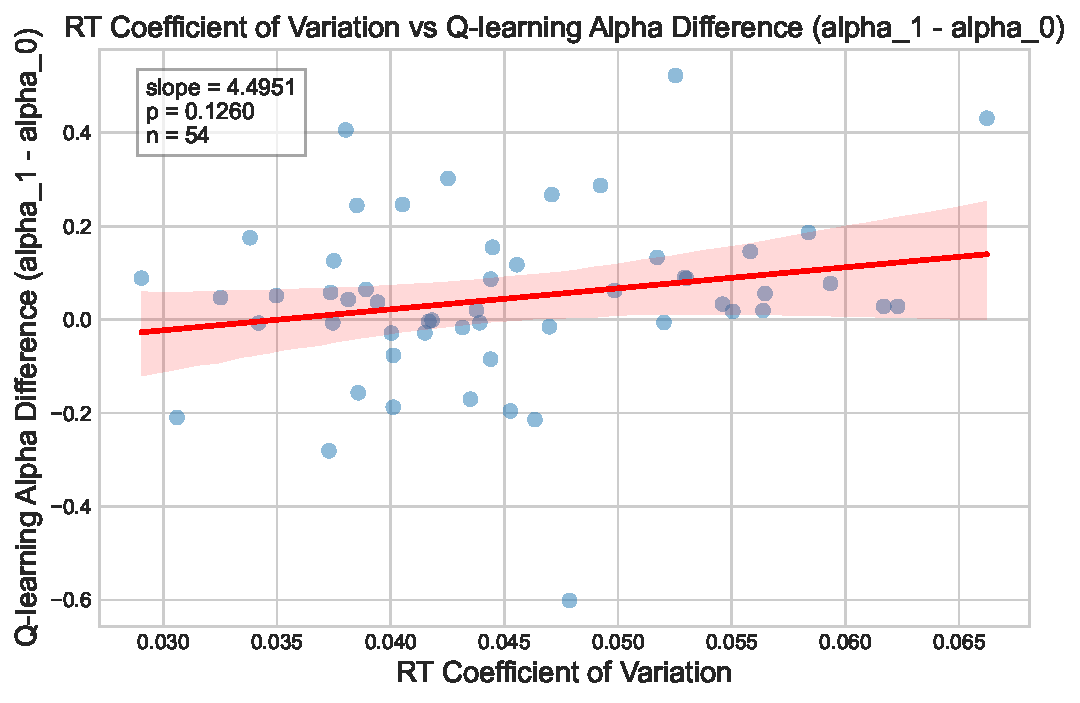
\includegraphics[width=0.8\textwidth]{../fig/rt_cv_vs_alpha_diff.pdf}
    \caption{学習の進行度合いの指標と反応時間の変動係数との関係．}
    \label{fig:rt_cv_vs_alpha_diff}
\end{figure}
最後に，$\Delta\alpha$ を学習の進行度合いの指標とし，反応時間の変動係数（${\text{CV}}_{\text{RT}}$）との関係を検討した．
その結果，学習率の差分と反応時間の変動との間に有意な関係は認められなかった（図~\ref{fig:rt_cv_vs_alpha_diff}）．


\section{\textcolor{red}{議論}}
本報告では，試行レベルの注意変動が暗黙的学習を媒介している可能性を検討した．
その結果，OOZ状態における学習率がNon-OOZ状態よりも高い方向の傾向が認められたが（$p = 0.07$），
学習率の差分と反応時間の変動係数との間に有意な関係は確認されなかった．

学習率がOOZ状態で高くなる傾向の解釈には，OOZ判定の二条件を踏まえる必要がある．
OOZ判定では，反応時間の水準が低くかつ局所的な変動が大きい試行が散漫状態として抽出される．
水準が低いという条件は，先行研究~\cite{decker2023pay}の定義に従えば，
熟慮を経ない衝動的な応答が生じた試行を選択的に拾うことを意味する．
このとき刺激に対する選択的処理が弱まることで，一方のドット群への注意の絞り込みが緩み，
両方の刺激情報と報酬フィードバックの随伴関係がより広く符号化される可能性がある．
すなわち，知覚精度を犠牲にしながらも報酬構造の学習に対する入力が広がることで，
学習率が上昇する方向に作用していると解釈できる．
このような注意の絞り込みの緩和が暗黙的学習を促進するという解釈は，
近年のマインドワンダリング研究と整合する．
Simorら~\cite{simor2025mind}は，マインドワンダリングが注意の範囲を広げることで，
課題のルールや目標が明示的でない状況において，
環境中の確率的な随伴関係の探索を促進する可能性を指摘している．
ただし，本研究で用いた課題は知覚判断を伴う応答であり，
先行研究のような単純な応答課題と比較して，散漫状態における反応時間の方向性が自明ではない．
そのため，本課題において速い応答が散漫状態に対応するかどうかは別途検証が必要である．

一方で，学習率の差分が反応時間の変動係数と関連しなかったことは，
試行レベルの注意状態と個人レベルの注意特性が異なる成分を反映している可能性を示している．
OOZ判定は反応時間の変動のうち速い側の局所的な揺らぎのみを選択的に抽出する指標であるのに対し，
反応時間の変動係数は遅い側の変動や状態のゆるやかな遷移を含む全体的な不安定性を反映する．
そのため，OOZ判定を経由した学習指標は，反応時間の変動係数が捉えている学習関連成分を必ずしも捕捉しているとは限らない．

以上の結果は，試行レベルの注意変動（OOZ）と個人レベルの注意特性（反応時間の変動係数）が，
暗黙的学習に対して独立に寄与している可能性を示唆している．

\clearpage
\bibliographystyle{unsrt}
\bibliography{myrefs}

\end{document}